\documentclass[tikz]{standalone}

% Required packages
\usepackage[utf8]{inputenc}
\usepackage[T1]{fontenc}
\usepackage{lmodern} % For smooth fonts
\usepackage{amsmath} % For math symbols like \forall and \in
\usepackage{tikz}

% TikZ libraries for advanced features
\usetikzlibrary{
    positioning,      % For placing nodes relative to each other (e.g., right=of)
    decorations.pathreplacing, % For drawing curly braces
    arrows.meta,      % For modern arrow tips (e.g., Stealth)
    calc              % For calculating coordinates (e.g., midpoints)
}

\begin{document}
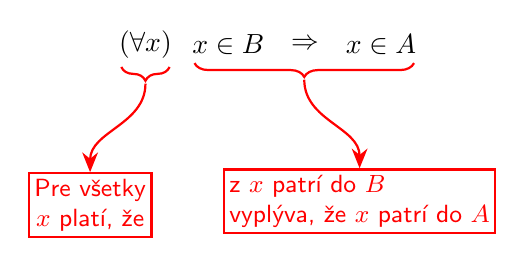
\begin{tikzpicture}[
    % Global style settings
    node distance=0.8em and 1.5em, % Default vertical and horizontal spacing for nodes
    % Style for the red elements
    red_style/.style={
        color=red, 
        thick
    },
    % Style for arrowheads
    arrow_tip/.style={
        -{Stealth[length=2.5mm, width=2mm]}
    },
    % Style for the text labels (smaller font, boxed)
    label_style/.style={
        draw, % This adds the box around the node
        font=\sffamily\small, % Use a small, sans-serif font
        inner sep=2pt, % Add a little padding inside the box
        align=left % Align text to the left for multi-line boxes
    }
]
    % 1. Define the nodes for the main formula.
    \node[inner sep=1pt] (quantifier) {$(\forall x)$};
    \node[inner sep=1pt, right=0.5em of quantifier] (x_in_B) {$x \in B$};
    \node[right=0.5em of x_in_B] (implies) {$\Rightarrow$};
    \node[inner sep=1pt, right=0.5em of implies] (x_in_A) {$x \in A$};

    % 2. Place the annotation text nodes.
    % Shifted 'quant_text_down' to the left.
    \node[red_style, label_style, below=4em of quantifier, xshift=-2em, align=center] (quant_text_down) {Pre všetky \\ $x$ platí, že};
    
    % The second label spans under 'x in B => x in A'
    \coordinate (impl_start) at (x_in_B.south west);
    \coordinate (impl_end) at (x_in_A.south east);
    \coordinate (impl_midpoint) at ($(impl_start)!0.5!(impl_end)$);
    % Shifted 'impl_text_down' to the right.
    \node[red_style, label_style, below=4em of impl_midpoint, xshift=2em, align=left]
    (impl_text_down) {z $x$ patrí do $B$ \\ vyplýva, že $x$ patrí do $A$};

    % 3. Draw the decorative curly braces (all red, pointing upwards, with small gap).
    \draw[red_style, decorate, decoration={brace, amplitude=5pt, mirror, raise=2pt}]
        ([xshift=2pt]quantifier.south west) -- ([xshift=-2pt]quantifier.south east);
    
    \draw[red_style, decorate, decoration={brace, amplitude=5pt, mirror, raise=2pt}]
        ([xshift=2pt]x_in_B.south west) -- ([xshift=-2pt]x_in_A.south east);

    % 4. Draw the arrows with double bends and vertical angles.
    \draw[red_style, arrow_tip] ($(quantifier.south)-(0,8pt)$) to[out=-90, in=90] (quant_text_down.north);
    \draw[red_style, arrow_tip] ($(impl_midpoint)-(0,8pt)$) to[out=-90, in=90] (impl_text_down.north);

\end{tikzpicture}
\end{document}
